\documentclass[handout]{beamer}

\usepackage{algorithm,algorithmic}
\usepackage{amsmath}
\usepackage{biblatex}
\usepackage{amsmath,mathtools}
\usepackage{physics}
\graphicspath{{../assets/}}
\addbibresource{bibliography.bib}

\parskip=10pt
\newcommand{\arctanh}{\text{arctanh}}
\newcommand{\reqeq}{\overset{!}{=}}

\newcommand{\myvec}[1]{\ensuremath{\begin{pmatrix}#1\end{pmatrix}}}

\usetheme{CambridgeUS}

\title{Complex Networks}
\author{Shoichi Yip}
\institute{M2 PCS}
\date{3 April 2024}

\begin{document}

\frame{\titlepage}

\section{Random graphs of the configuration model}

\begin{frame}{Complex networks}
    \alert{Networks} are often the backbone of many complex systems.

    Biological systems, citations in papers, social networks can be all modeled
    as complex networks.

    The modeling of complex networks has stem from the study of
    \alert{models of random graphs}, starting with the pioneering work by Paul
    Erd\H{o}s and Alfr\'{e}d R\'{e}nyi in 1959.
\end{frame}

\begin{frame}{Random graphs}
\end{frame}

\begin{frame}{The problem with ER graphs}
    Graphs generated using the ER model have a Poisson degree distribution.

    However, experimental study of real world graphs show us that most of the
    times they do not follow a Poissonian behaviour.

    We can overcome this problem by using the \alert{configuration model}.
\end{frame}

\begin{frame}{The configuration model}
    The \alert{configuration model} allows us to generate graphs exactly with a
    given \alert{degree sequence} $\vec k$.

    The degree sequence is a vector, for example,
    $$
    \vec k = \myvec{3 & 2 & 3 & 1 & 1}
    $$
    where each $i$-th element is the degree of the $i$-th node.
\end{frame}

\begin{frame}{Sampling a graph from a configuration model}
    The configuration model provides us with a constructive algorithm in order
    to find an instance of a random graph, provided a degree sequence $\vec k$.

    For example, if we take the $\vec k$ degree sequence from the previous slide
    we can start with a set of unconnected nodes where each $i$-th node has
    $k_i$ \alert{stubs}, or half-edges.

    Then we get a random graph instance by taking two random stubs at a time and
    connecting them. On general grounds, the configuration model allows for the
    presence of multiple edges and self-edges.
\end{frame}

\begin{frame}{Sampling a graph from a configuration model}
    \begin{figure}
        \centering
        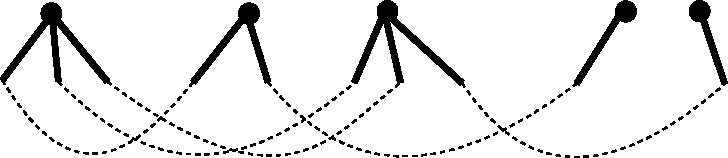
\includegraphics[width=.4\textwidth]{config_model}
        \caption{Connecting stubs in the configuration model}
        \label{fig:config_model}
    \end{figure}
\end{frame}

\begin{frame}{Configuration model given a degree distribution}
    We can adapt the configuration model to a specific task, that of sampling
    graphs that have a specific \alert{degree distribution}.

    We can in fact first of all define a degree sequence such that the abundance
    of nodes of degree $d$ are given by a degree distribution $p_d$. Then we can
    proceed as we would do for the configuration model, by wiring the stubs.

    We can hence extract random graph instances that nearly exactly match the
    degree distribution.
\end{frame}

\begin{frame}{Our ensemble}
    In our particular case, we define a random graph ensemble $\mathcal{G}$ such
    that:
    \begin{itemize}
        \item the graph has $N$ nodes;
        \item the graph is generated using the configuration model;
        \item the graph \alert{does not} contain self-edges and multiple edges;
        \item we define a parameter $\pi$ and the the graph is such that the
            fraction of the nodes $p_1 = 1-\pi$ has degree 1, and the remaining
            fraction $p_4 = \pi$ has degree 4.
    \end{itemize}
\end{frame}

\begin{frame}{Algorithm to generate RG instance}
    \begin{algorithm}[H]
        \begin{algorithmic}[1]
            \FOR{$k_i$ in degree sequence $\vec k$}
                \STATE Generate node with $k_i$ stubs
            \ENDFOR
            \WHILE{Graph $G$ not generated}
                \WHILE{Stub list is not exhausted}
                    \STATE Pick two random stubs
                    \STATE Create a candidate edge between them
                    \STATE Check whether they are not multiedge or self-edge
                \ENDWHILE
            \ENDWHILE
        \end{algorithmic}
        \caption{Algorithm to generate stubs and connect them}
    \end{algorithm}
\end{frame}

\begin{frame}{Examples of random graphs}
    \begin{figure}
        \centering
        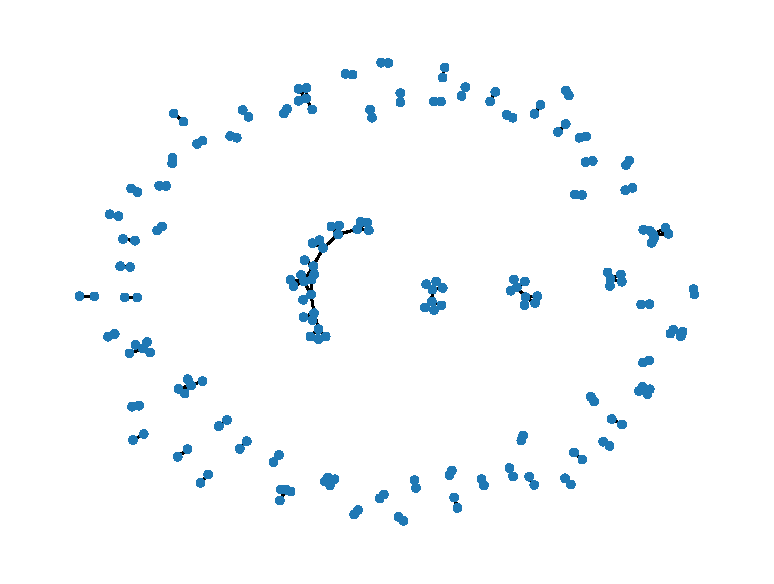
\includegraphics[height=.7\textheight]{rg0}
        \caption{Instance of a random graph for $\pi=0.1$}
        \label{fig:rg0}
    \end{figure}
\end{frame}

\begin{frame}{Examples of random graphs}
    \begin{figure}
        \centering
        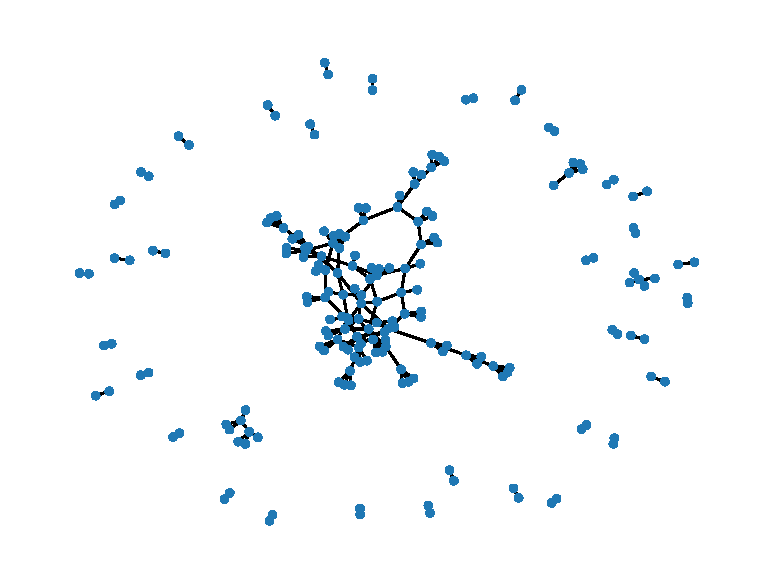
\includegraphics[height=.7\textheight]{rg1}
        \caption{Instance of a random graph for $\pi=0.3$}
        \label{fig:rg1}
    \end{figure}
\end{frame}

\begin{frame}{Examples of random graphs}
    \begin{figure}
        \centering
        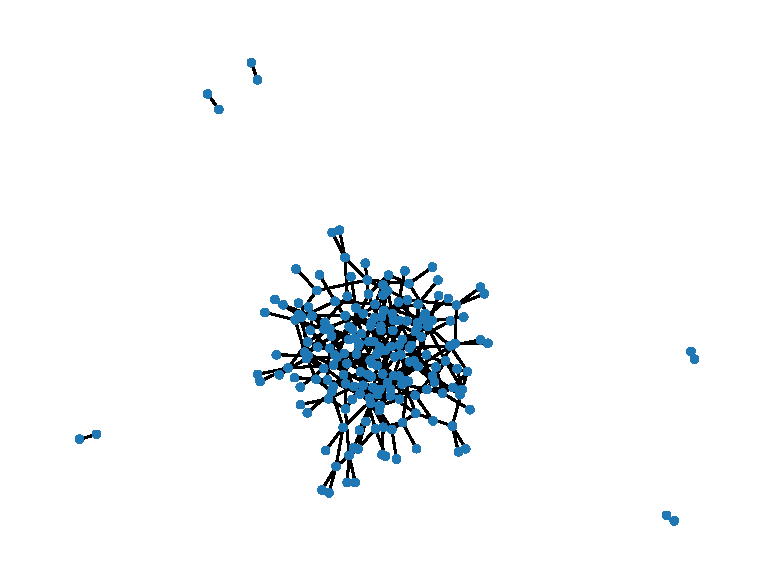
\includegraphics[height=.7\textheight]{rg2}
        \caption{Instance of a random graph for $\pi=0.7$}
        \label{fig:rg2}
    \end{figure}
\end{frame}

\section{The giant component}

\begin{frame}{The giant component}
\end{frame}

\begin{frame}{Detecting the giant component in an instance}
    We explore the connected components with a \alert{Breadth-First Search}
    (BFS) algorithm \ref{algo:bfs}.

    Once all connected components have been detected, they are stored in a
    dictionary-like object and the size of the biggest is given as an output.
\end{frame}

\begin{frame}{BFS algorithm}
    \begin{algorithm}[H]
        \begin{algorithmic}[1]
            \STATE All nodes are unvisited
            \WHILE{Set of unvisited nodes is nonempty}
                \STATE Initialize queue with unvisited node
                \WHILE{Queue is nonempty}
                    \STATE Assign last node of queue to component $t$
                    and remove from the queue
                    \FOR{All neighbours of the node}
                        \IF{The neighbour doesn't belong to component $t$}
                            \STATE Add to component $t$
                            \STATE Add to queue
                        \ENDIF
                    \ENDFOR
                \ENDWHILE
            \ENDWHILE
        \end{algorithmic}
        \caption{Breadth-First Search algorithm implementation}
        \label{algo:bfs}
    \end{algorithm}
\end{frame}

\begin{frame}{The onset of criticality}
    On an intuitive ground, we can argue that in an ER graph the number of nodes
    visited after a $k$ steps walk is on average given by $c^k=e^{k\log{c}}$.
    Then for $c<1$ the number gets smaller and smaller while for $c>1$ it
    becomes extensive.

    On the same line of reasoning, we can replace $c$ with the average number of
    nearest neighbours which is given by the average excess degree, hence we get
    that the onset of criticality happens for
    \begin{equation}
        \frac{\expval{d^2} - \expval{d}}{\expval{d}} \reqeq 1
        \label{eq:onset_condition}
    \end{equation}
\end{frame}

\begin{frame}{The onset of criticality}
    Then
    $$
    \expval{d^2} - 2\expval{d} \reqeq 0
    $$
    which in our case is given by
    $$
    (1-\pi) + 16 \pi - 2 [(1-\pi) + 4 \pi] \reqeq 0
    $$

    The final result is that the criticality threshold is given by
    \begin{equation}
        \pi = \frac{1}{9}
    \end{equation}
\end{frame}

\begin{frame}{Size of the giant component}
    In order to find the size of the giant component we resort to the study of
    the probability that an excess node or a node belongs to the giant
    component \cite[56]{weigt}.

    \begin{figure}
        \centering
        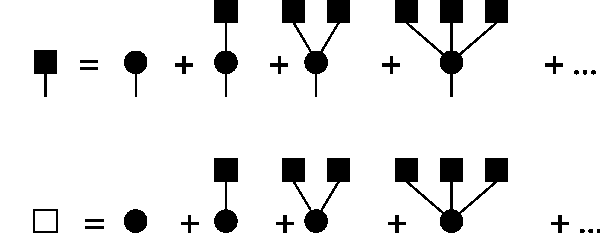
\includegraphics[width=.6\textwidth]{PTCOP_iterative}
        \caption{Scheme for the iterative solution to find the probability that
        a node belongs to the giant component and the excess probability}
        \label{fig:iterative}
    \end{figure}
\end{frame}

\begin{frame}{Excess probability that node belongs to GC}
    The scheme reads as follows. The excess proability $\mu$, which is
    the probability that given a randomly selected edge one of its end vertices
    is not connected with a GC, is given by
    \begin{itemize}
        \item the probability that the excesss node has degree 1, i.e. there
            would not exist any other edge that connects it to a GC
        \item the probability that the excess node is connected to a node that
            does not belong to the GC
        \item the probability that the excess node is connected to two nodes
            that do not belong to the GC
        \item etc.
    \end{itemize}
\end{frame}

\begin{frame}{Probability that node belongs to GC}
    The same goes for the probability that a randomly selected node does not
    belong to the GC. The proability $1-\gamma$, is given by
    \begin{itemize}
        \item the probability that this node is isolated
        \item the probability that this node is connected to a node that does
            not belong to the GC
        \item the probability that this node is connected to two nodes that do
            not belong to the GC
        \item etc.
    \end{itemize}
\end{frame}

\begin{frame}{Iterative equations}
    We then find the iterative equations, respectively
    \begin{equation}
        \begin{cases}
            \mu = q_1 + q_2 \mu + q_3 \mu^2 + ...\\
            1 - \gamma = p_0 + p_1 \mu + p_2 \mu^2 + ...
        \end{cases}
        \label{eq:iterative}
    \end{equation}

    Since our degree distribution has only two nonzero terms for $d=1$ and
    $d=4$, we can rewrite them as
    \begin{equation}
        \begin{cases}
            \mu = q_1 + q_4 \mu^3\\
            1 - \gamma = p_1 \mu + p_4 \mu^4
        \end{cases}
        \label{eq:iterative_cm}
    \end{equation}
    where
    $$
    q_1 = \frac{1-\pi}{1+3\pi} \qquad q_4 = \frac{4\pi}{1+3\pi}
    $$
\end{frame}

\begin{frame}{}
    We can solve the first third order equation in Eq.~\ref{eq:iterative_cm} and
    we get
    $$
    \mu = 1 \quad \lor \quad \mu = \frac{-1-\sqrt{\pi}}{2\sqrt{\pi}} \quad
    \lor \quad \mu = \frac{1-\sqrt{\pi}}{2\sqrt{\pi}}
    $$
    where the first solution is the trivial solution that does not have any
    giant component, and the second solution is negative (so it cannot be a
    probability). If we plug the third solution in the second equation we get
    \begin{equation}
        \gamma = 1 - (1-\pi) \frac{1-\sqrt{\pi}}{2\sqrt{\pi}} - \pi \left(
        \frac{1-\sqrt{\pi}}{2\sqrt{\pi}} \right)^4
        \label{eq:gamma_final}
    \end{equation}
    which gives us the theoretical value of the probability of a node being part
    of the GC, hence also the expectation value over the size of the GC.
\end{frame}

\begin{frame}{The size of the giant component}
    \begin{figure}
        \centering
        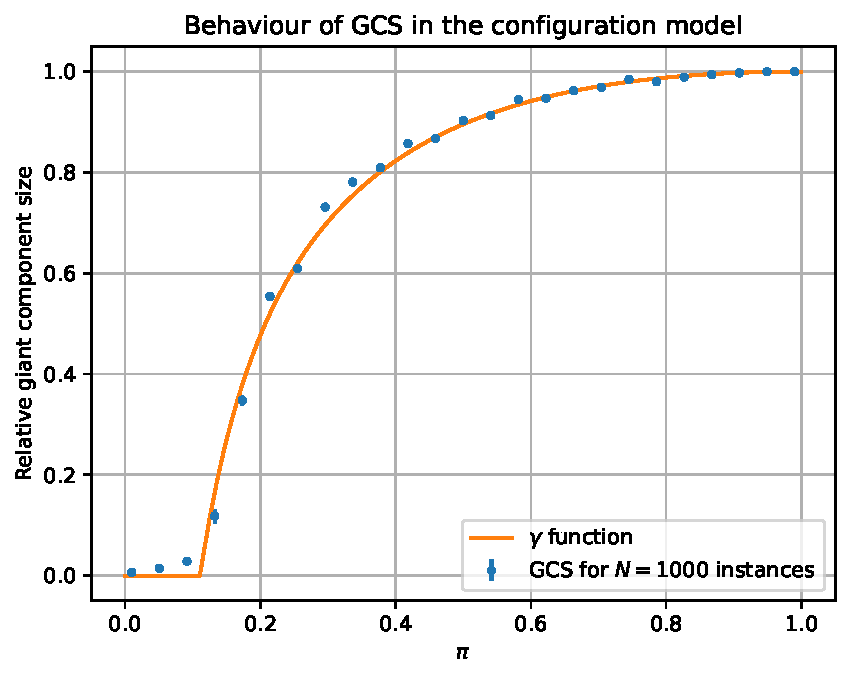
\includegraphics[height=.7\textheight]{gcs}
        \caption{Comparison between theoretical value and measures from random
        instances of the size of the giant component}
        \label{fig:gcs}
    \end{figure}
\end{frame}

\section{Emergence of $q$-cores}

\begin{frame}{The deterministic $q$-core algorithm}
    The $q$-core of a graph can be found using a simple algorithm.

    \begin{algorithm}[H]
        \begin{algorithmic}[1]
            \WHILE{Nodes with $d < q$ are present}
                \STATE Remove all nodes with $d<q$
            \ENDWHILE
        \end{algorithmic}
        \caption{Algorithm for deterministic $q$-core detection}
        \label{algo:qcore_det}
    \end{algorithm}

    We will use this algorithm to find the size of a $q$-core.
\end{frame}

\begin{frame}{The stochastic $q$-core algorithm}
    There is a stochastic version of this algorithm.

    \begin{algorithm}[H]
        \begin{algorithmic}[1]
            \WHILE{Nodes with $d < q$ are present}
            \STATE{Select randomly a node with degree $d < q$}
            \IF{The node has degree $d < q$}
            \STATE{Remove node}
            \ENDIF
            \ENDWHILE
        \end{algorithmic}
        \caption{Algorithm for stochastic $q$-core detection}
        \label{algo:qcore_stoc}
    \end{algorithm}

    This algorithm does not remove an extensive amount of nodes for each
    timestep and its dynamic can be described by an ODE.
\end{frame}

\begin{frame}{Rate equations for the $q$-core}
    The behaviour of $q$-cores in Algorithm~\ref{algo:qcore_stoc} can be
    described by \alert{rate equations} using the \alert{Wormwald method}.
    \cite[58]{weigt}.

    The algorithmic time $N(T) = N - T$ describes the amount of nodes that are
    still available, where $N$ is the total number of nodes and $T$ is the
    number of nodes that we have removed.

    We can introduce a \alert{rescaled time} $t = T / N$, which will span from 0
    to 1.

    The variable that we want to study in time is the \alert{degree
    distribution at time $t$}
    \begin{equation}
        p_d(t) = \frac{N_d(t)}{N(t)} = \frac{N_d(t)}{N[1-t]}
        \label{eq:deg_time}
    \end{equation}
\end{frame}

\begin{frame}{ODE for the rate equation}
    We can write the difference between two consecutive timesteps of the number
    of nodes of degree $d$ as
    \begin{equation}
        N_d(T+1) - N_d(T) =
        - \frac{\chi_d p_d}{\overline \chi_d}
        + \frac{\overline{\chi_d d}}{\overline \chi_d c(t)}
        [(d+1) p_{d+1}(t) - dp_d(t)]
        \label{eq:diff_ndeg}
    \end{equation}
    where $\chi_d$ is the \alert{indicator function}
    \begin{equation}
        \chi_d =
        \begin{cases*}
            1 & if $d<q$\\
            0 & if $d\geq q$
        \end{cases*}
        \label{eq:indfunc}
    \end{equation}
    and $c(t)$ is the average connectivity at time $t$
    \begin{equation}
        c(t) = \sum_d d p_d(t)
        \label{eq:avgcon}
    \end{equation}
\end{frame}

\begin{frame}{ODE for the rate equation}
    Starting from Eq.~\ref{eq:diff_ndeg} we can find the equations for $p_d(t)$
    \begin{equation}
        \partial_t[(1-t) p_d(t)] = - \frac{\chi_d p_d}{\overline \chi_d}
        + \frac{\overline{d \chi_d}}{c(t) \overline \chi_d}
        [(d+1) p_{d+1}(t) - d p_d(t)]
        \label{eq:wormwald_ode}
    \end{equation}
    
    Since we \alert{start} with finite $p_d(0)$ for $d=1,4$, we will have
    nonzero terms for $t>0$ for $d=0,1,2,3,4$. In fact, by randomly removing a
    node and its attached edges, we might decrease the degrees of its previously
    attached nodes.
\end{frame}

\begin{frame}{ODE for the rate equation}
    For our specific problem, if we define
    $$
    A(t) = \frac{1}{p_0(t) + p_1(t) + p_2(t)}
    \quad B(t) = \frac{p_1(t) + 2 p_2(t)}{c(t)} A(t)
    $$
    we get the system of equations
    {\scriptsize
    \begin{align*}
        \dv{p_0(t)}{t} &= \frac{1-A(t)}{1-t} p_0(t) + \frac{B(t)}{1-t} p_1(t)\\
        \dv{p_1(t)}{t} &= \frac{1-A(t)-B(t)}{1-t} p_1(t) + \frac{2B(t)}{1-t} p_2(t)\\
        \dv{p_2(t)}{t} &= \frac{1-A(t)-2B(t)}{1-t} p_2(t) + \frac{3B(t)}{1-t}
        p_3(t)\\
        \dv{p_3(t)}{t} &= \frac{1-3B(t)}{1-t} p_3(t) + \frac{4B(t)}{1-t} p_4(t)\\
        \dv{p_4(t)}{t} &= \frac{1-4B(t)}{1-t} p_4(t)
    \end{align*}
    where
    $$
    p_0(0) = 0 \quad p_1(0) = 1-\pi \quad p_2(0)=0 \quad p_3(0)=0 \quad
    p_4(0)=\pi
    $$
    }
\end{frame}

\begin{frame}{ODE for the rate equation}
    We can rephrase the ODE as
    \begin{equation}
        \dv{\vec p(t)}{t} = M(t) \vec p(t)
        \label{eq:ode_compact}
    \end{equation}
    where
    {\scriptsize
    $$
    M(t) = \frac{1}{1-t}
    \begin{pmatrix}
        1-A(t) & B(t) & 0 & 0 & 0\\
        0 & 1-A(t)-B(t) & 2B(t) & 0 & 0\\
        0 & 0 & 1-A(t)-2B(t) & 2B(t) & 0\\
        0 & 0 & 0 & 1-3B(t) & 4B(t)\\
        0 & 0 & 0 & 0 & 1-4B(t)
    \end{pmatrix}
    $$
    }

    Equation~\ref{eq:ode_compact} is an initial value problem and it can be
    solved numerically with the \alert{Runge-Kutta} method.
\end{frame}

\begin{frame}{Runge-Kutta method for the IVP}
    An IVP can be solved numerically with the \alert{Runge-Kutta} method. 

    For each timestep from $t$ to $t+h$ we can compute \cite{oderk} the function
    value as
    \begin{align}
        K_1 &= h f(t, u)\\
        K_2 &= h f(t + h/2, u + K_1/2)\\
        K_3 &= h f(t + h/2, u + K_2/2)\\
        K_4 &= h f(t + h, u + K_3)\\
        u(t+h) &\approx u + \frac{1}{6}(K_1 + 2 K_2 + 2 K_3 + K_4)
    \end{align}
\end{frame}

\begin{frame}{Example of the ODE: $\pi=0.3$}
    \begin{figure}
        \centering
        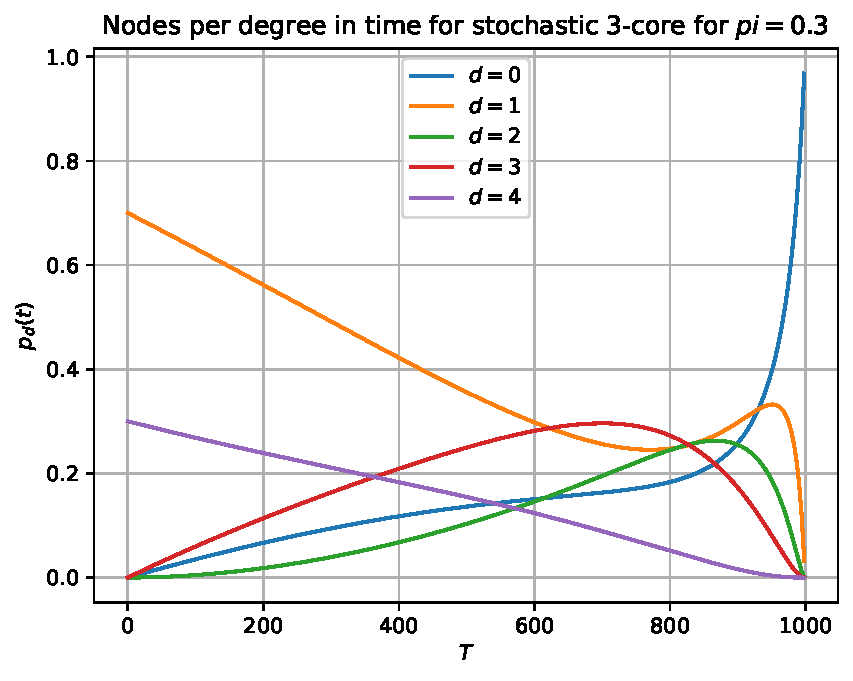
\includegraphics[width=.6\textwidth]{ode_evol_pi03.pdf}
        \caption{Evolution of the ODE for $\pi=0.3$}
        \label{ref:ode_evol_pi03}
    \end{figure}
\end{frame}

\begin{frame}{Example of the ODE: $\pi=0.8$}
    \begin{figure}
        \centering
        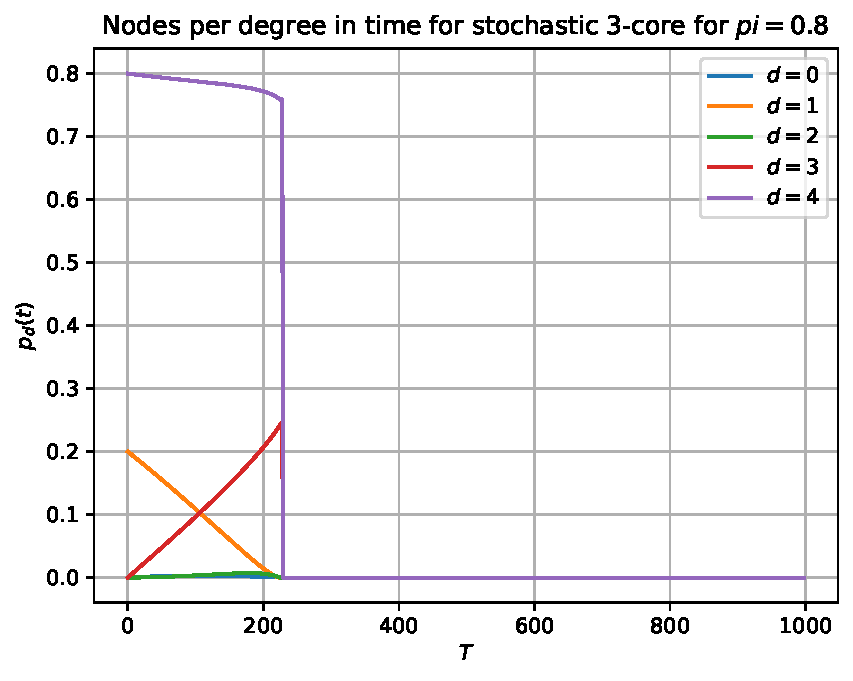
\includegraphics[width=.6\textwidth]{ode_evol_pi08.pdf}
        \caption{Evolution of the ODE for $\pi=0.8$, the time where all rates
        go to zero is the \emph{halting time} $T_f$}
        \label{ref:ode_evol_pi03}
    \end{figure}
\end{frame}

\begin{frame}{The size of the 3-core}
    \begin{figure}
        \centering
        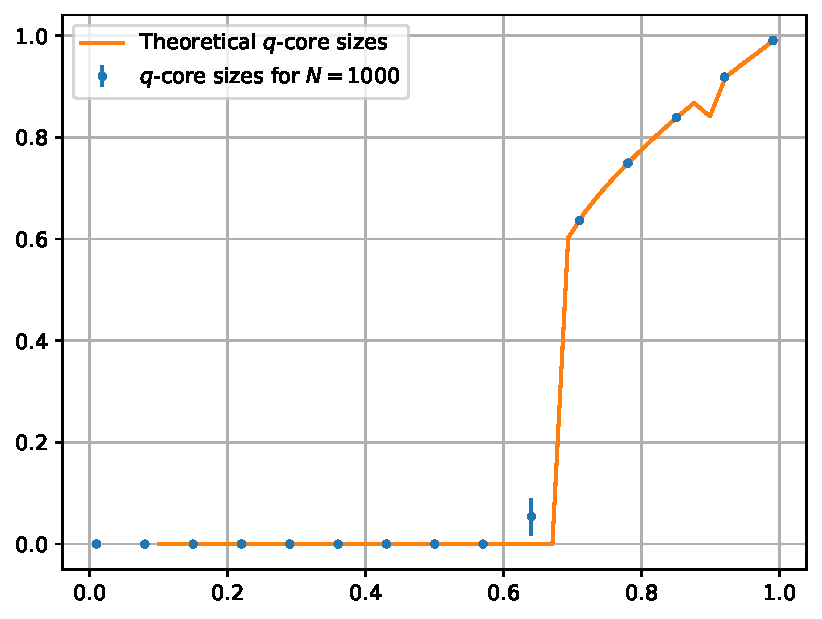
\includegraphics[height=.7\textheight]{qcore}
        \caption{Comparison between theoretical value and measures from random
        instances of the size of the 3-core}
        \label{fig:qcore}
    \end{figure}
\end{frame}

\section{The ferromagnetic Ising model}

\begin{frame}{The ferromagnetic Ising model}
    The \alert{ferromagnetic Ising model} is a model described on the graph
    structure. Its behaviour is described by the Hamiltonian
    \begin{equation}
        \mathcal{H} = -\sum_{(ij)\in E} \sigma_i \sigma_j
        \label{eq:ferroising_ham}
    \end{equation}
    where
    $$
        \sigma_i = \pm 1 \qquad \forall i \in 1, ..., N,
    $$
    $E$ is the edge set and $\sigma_i$ are binary values defined on the $i$-th
    node.
\end{frame}

\begin{frame}{What do we expect}
\end{frame}

\begin{frame}{MCMC}
    In order to simulate a ferromagnetic Ising model on a random graph sampled
    from $\mathcal{G}$, we might use \alert{Monte Carlo Markov Chains}.

    MCMCs are a class of algorithms that, given an equilibrium probability
    distribution, are able to converge to it using a Markov chain.

    The idea is that we are able, using a set of rules that satisfy detailed
    balance, to reach after a certain number of steps a satisfactory
    equilibrium configuration. \cite[31-42]{newman_barkema}.

    Usually these rules encode the information whether the new state is
    ``better'' or ``worse'' than the old one, and decide how to proceed.
\end{frame}

\begin{frame}{The Metropolis-Hastings algorithm}
    The \alert{Metropolis-Hastings} flips one spin per step and the difference
    in energy between configurations and the temperature of the system is
    evaluated in order to accept or reject the step. \cite[46]{newman_barkema}

    \begin{figure}
        \centering
        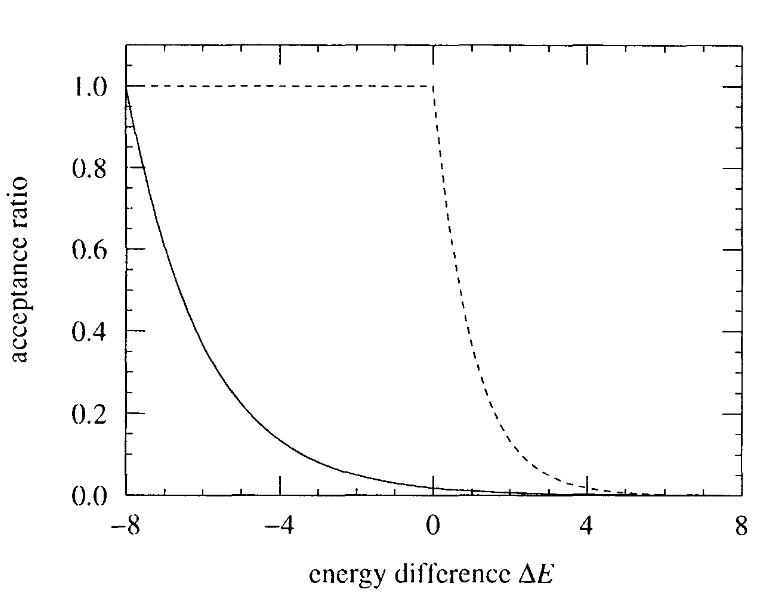
\includegraphics[width=.4\textwidth]{metropolis_acceptance.png}
        \caption{Metropolis-Hastings acceptance ratios (dashed line) from
        \cite[48]{newman_barkema}}
    \end{figure}
\end{frame}

\begin{frame}{The Metropolis-Hastings algorithm}
    \begin{algorithm}[H]
        \begin{algorithmic}[1]
            \STATE Initialize spins $\vec \sigma$
            \WHILE{System not at equilibrium}
                \STATE Choose a random $i$-th site
                \STATE Compute the $\Delta E =
                    \mathcal{H}(\vec\sigma^{\text{new}}) -
                    \mathcal{H}(\vec\sigma^{\text{old}})$
                \STATE Generate a random number $r\in [0,1]$
                \IF{$r<\exp(-\beta \Delta E)$}
                \STATE Flip the spin $\sigma_i^{\text{new}} =
                -\sigma_i^{\text{old}}$
                \ELSE
                    \STATE Do nothing
                \ENDIF
            \ENDWHILE
        \end{algorithmic}
        \caption{Metropolis-Hastings algorithm}
        \label{algo:metropolis}
    \end{algorithm}
\end{frame}

\begin{frame}{The Wolff algorithm}
    The \alert{Wolff algorithm} picks a random spin and probabilistically grows
    the cluster adding spins that are aligned. It then flips the entire cluster
    at once. \cite[91]{newman_barkema}

    \begin{figure}
        \centering
        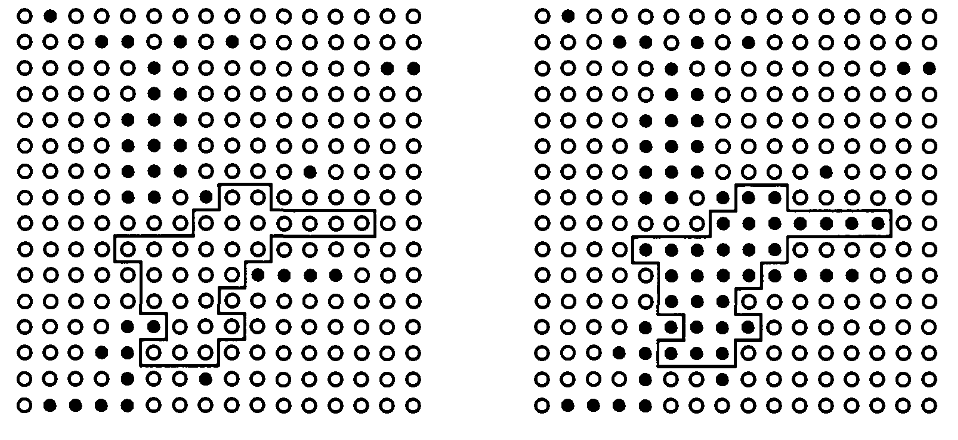
\includegraphics[width=.4\textwidth]{wolff.png}
        \caption{Cluster spin flip using Wolff algorithm from
        \cite[91]{newman_barkema}}
    \end{figure}
\end{frame}

\begin{frame}{The Wolff algorithm}
    The \alert{Wolff algorithm} picks a random spin and probabilistically grows
    the cluster adding spins that are aligned. It then flips the entire cluster
    at once. \cite[91]{newman_barkema}

    \begin{algorithm}[H]
        \begin{algorithmic}[1]
            \STATE Initialize spins $\vec \sigma$
            \WHILE{System not at equilibrium}
                \WHILE{Aligned neighbourhood is not exhausted}
                    \STATE Look at neighbours
                    \IF{They are aligned to the first spin}
                    \STATE Add to cluster with probability $P_{\text{add}} = 1-e^{-2\beta J}$
                    \ENDIF
                \ENDWHILE
                \STATE Flip the spins of the cluster
            \ENDWHILE
        \end{algorithmic}
        \caption{Wolff algorithm}
        \label{algo:wolff}
    \end{algorithm}
\end{frame}

\begin{frame}{Sampling equilibrium states of Ising on RG}
    We choose to use the \alert{Wolff algorithm} for speeding up the sampling
    also in the critical phase. The implementation is similar to the 2D Ising
    case, taking care of the definitions of neighbourhoods.

    Some runs over sets of $(\pi, T)$ parameters are performed in order to
    understand how much time does the system take to equilibrate in terms of
    magnetization $m=\sum_i \sigma_i / N$.

    After the equilibration time $\tau_{\text{eq}}$ has passed, the
    magnetization $m$ is measured every $\tau_{\text{sample}}$ steps. The
    samples are then averaged and yield the final result for each RG instance.
\end{frame}

\begin{frame}[plain]
    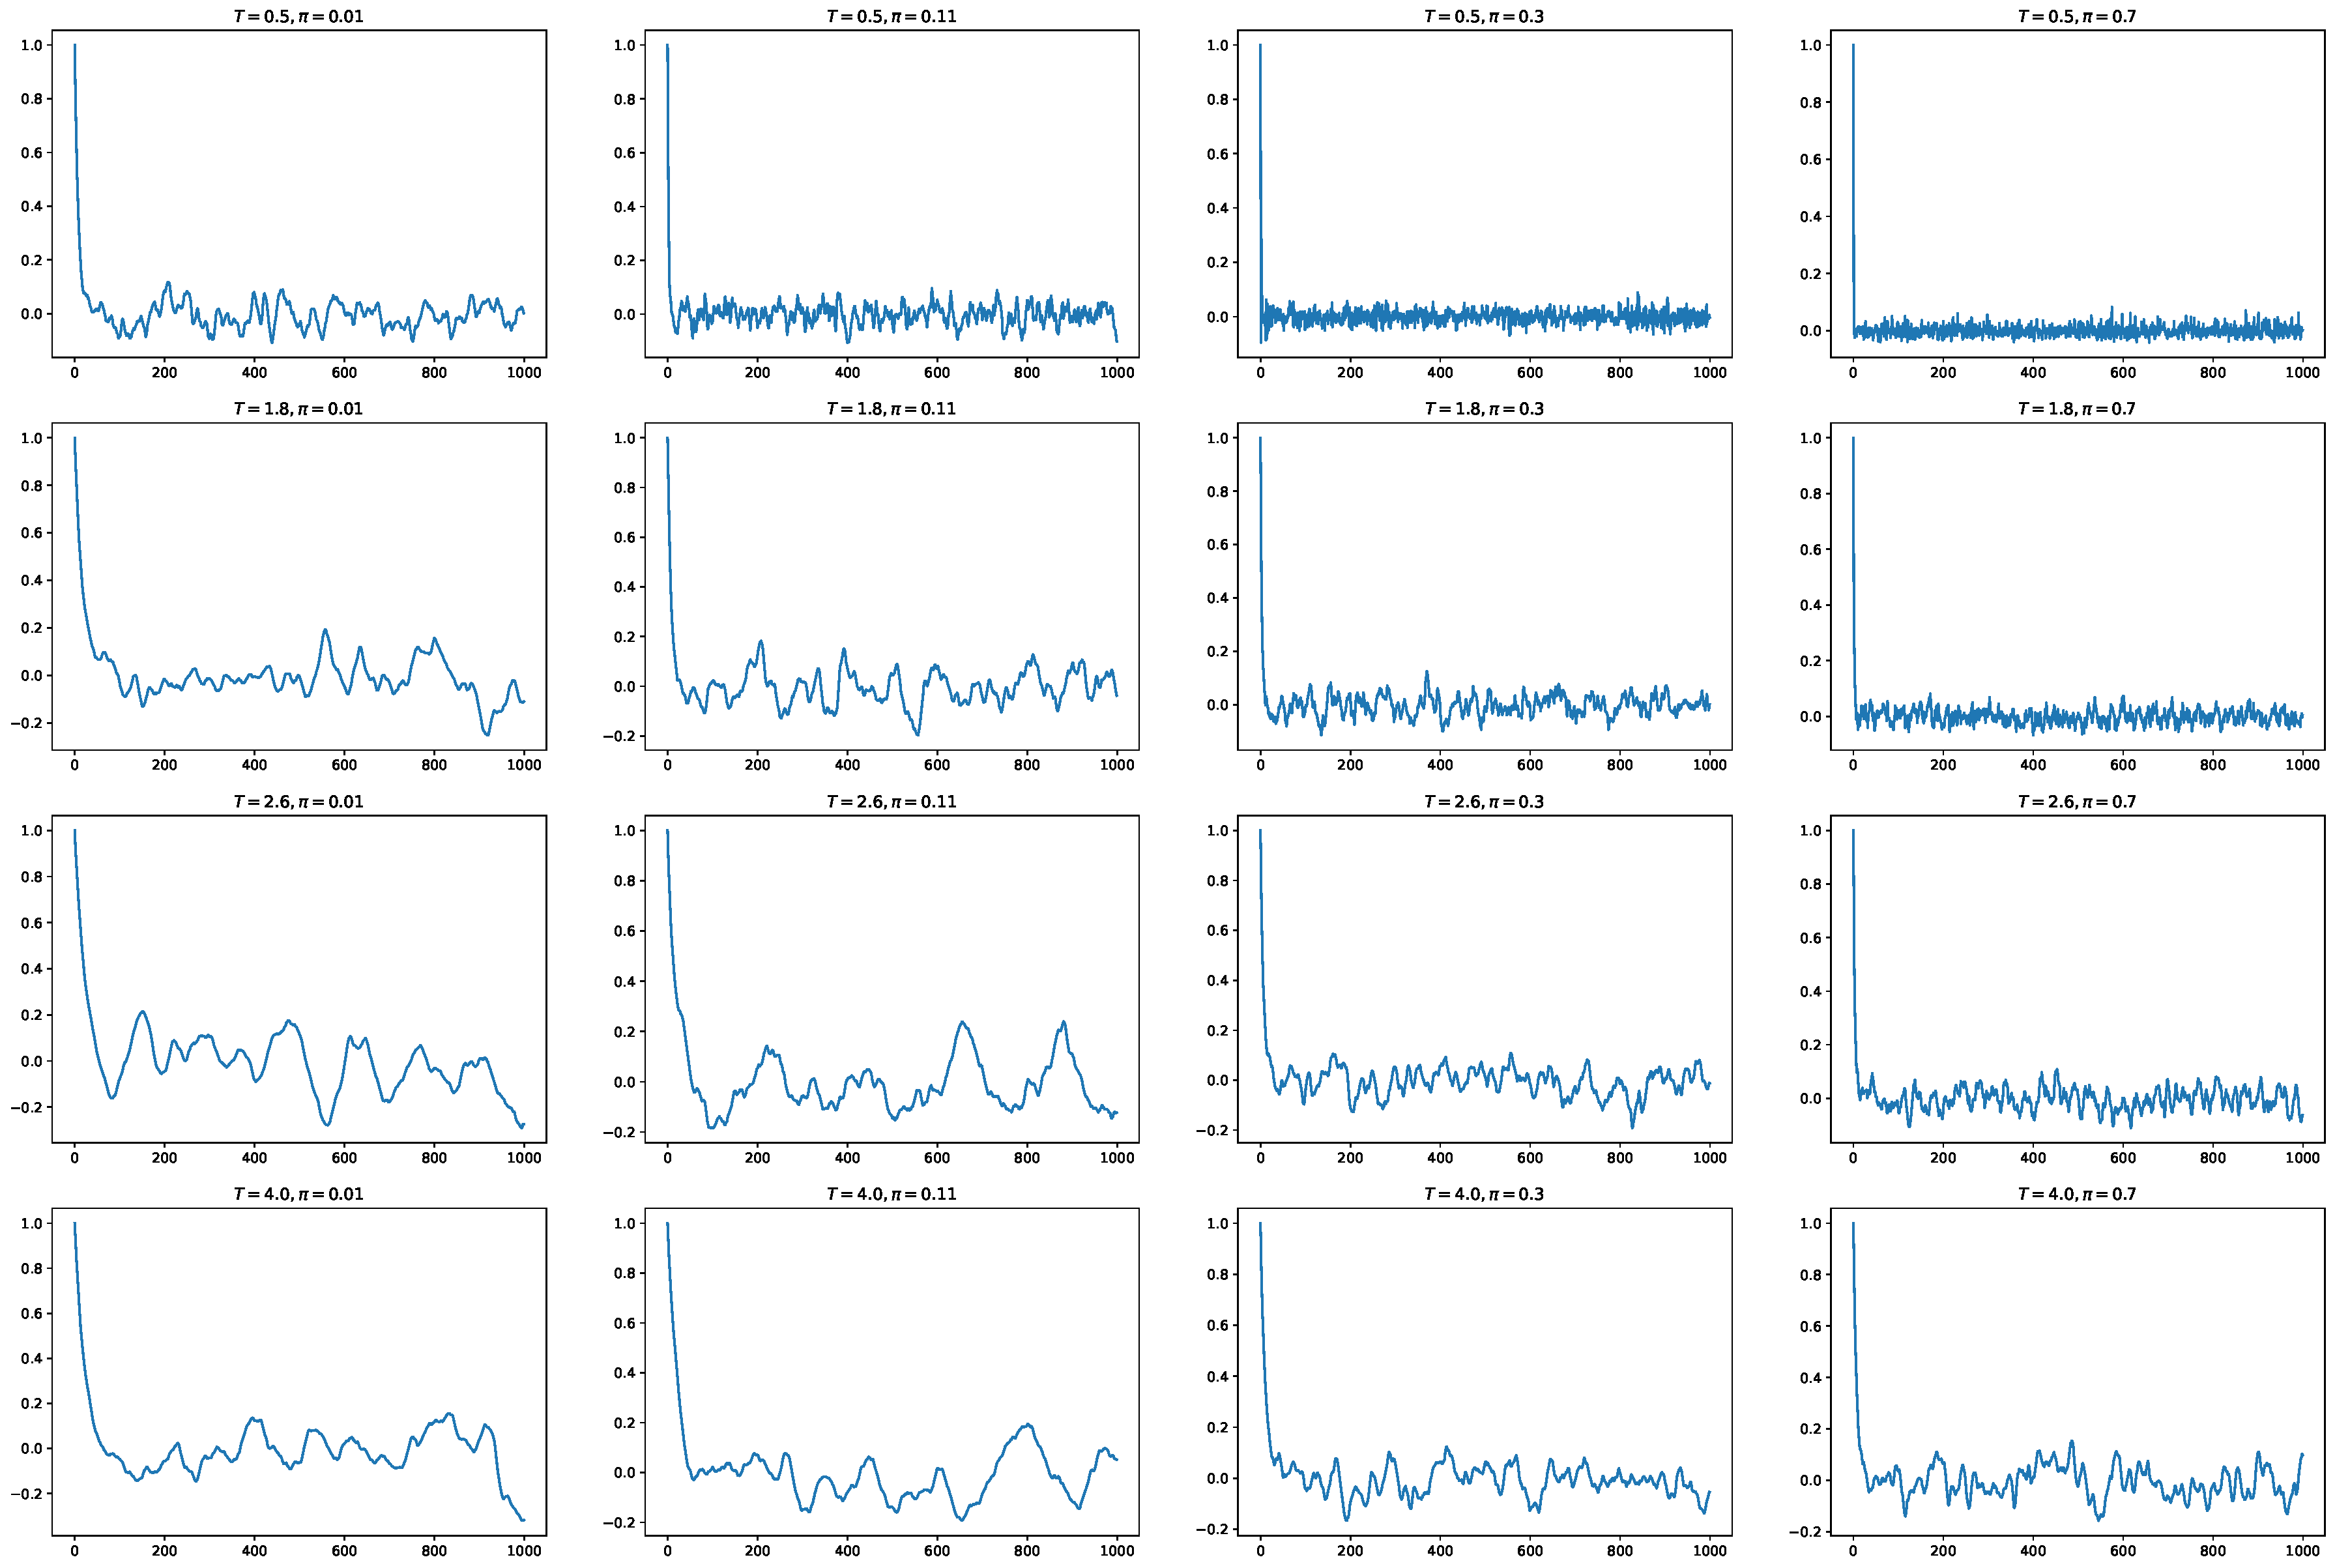
\includegraphics[width=\textwidth]{wolff_mags}
\end{frame}

\begin{frame}{Belief Propagation}
    Another way to study the Ising model is by using the \alert{belief
    propagation} equations.

    They are equations that are defined on tree-like graphs. These equations
    allow us to make an exact estimate of the local fields...
\end{frame}

\begin{frame}{Approximate Belief Propagation}
    The BP equations can also be applied to the case of graphs that have loops.
    In that case they are approximate equations, and
\end{frame}

\begin{frame}[plain]
    \begin{figure}
        \centering
        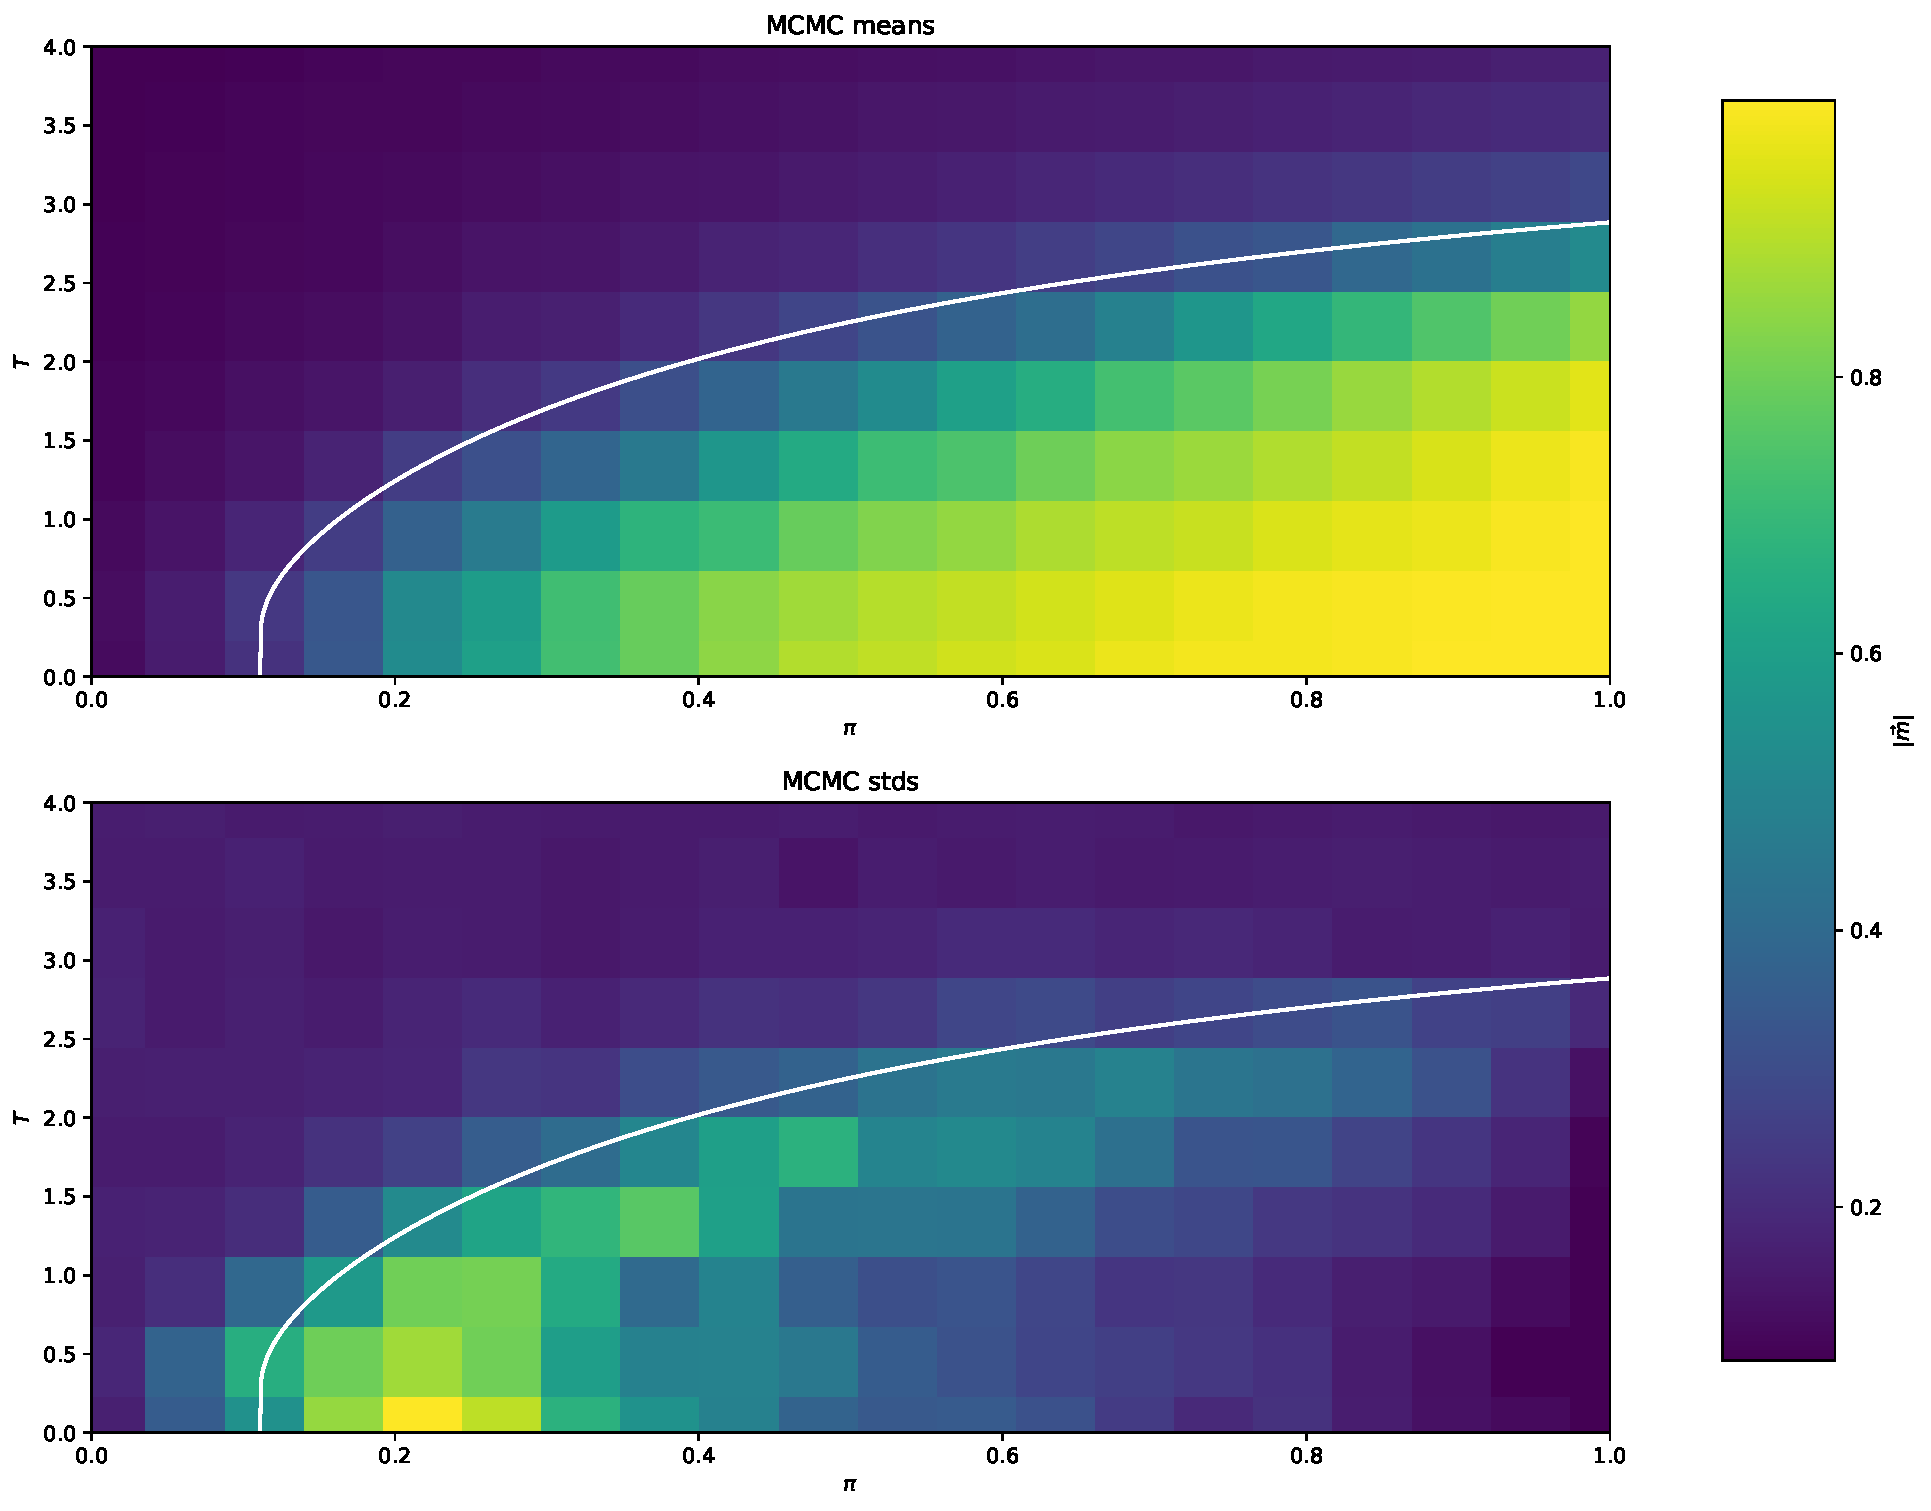
\includegraphics[width=.8\textwidth]{mcmc_heatmap}
        \caption{Heatmap for MCMC sampled magnetization means and stds}
        \label{fig:mcmc_heatmap}
    \end{figure}
\end{frame}

\begin{frame}[plain]
    \begin{figure}
        \centering
        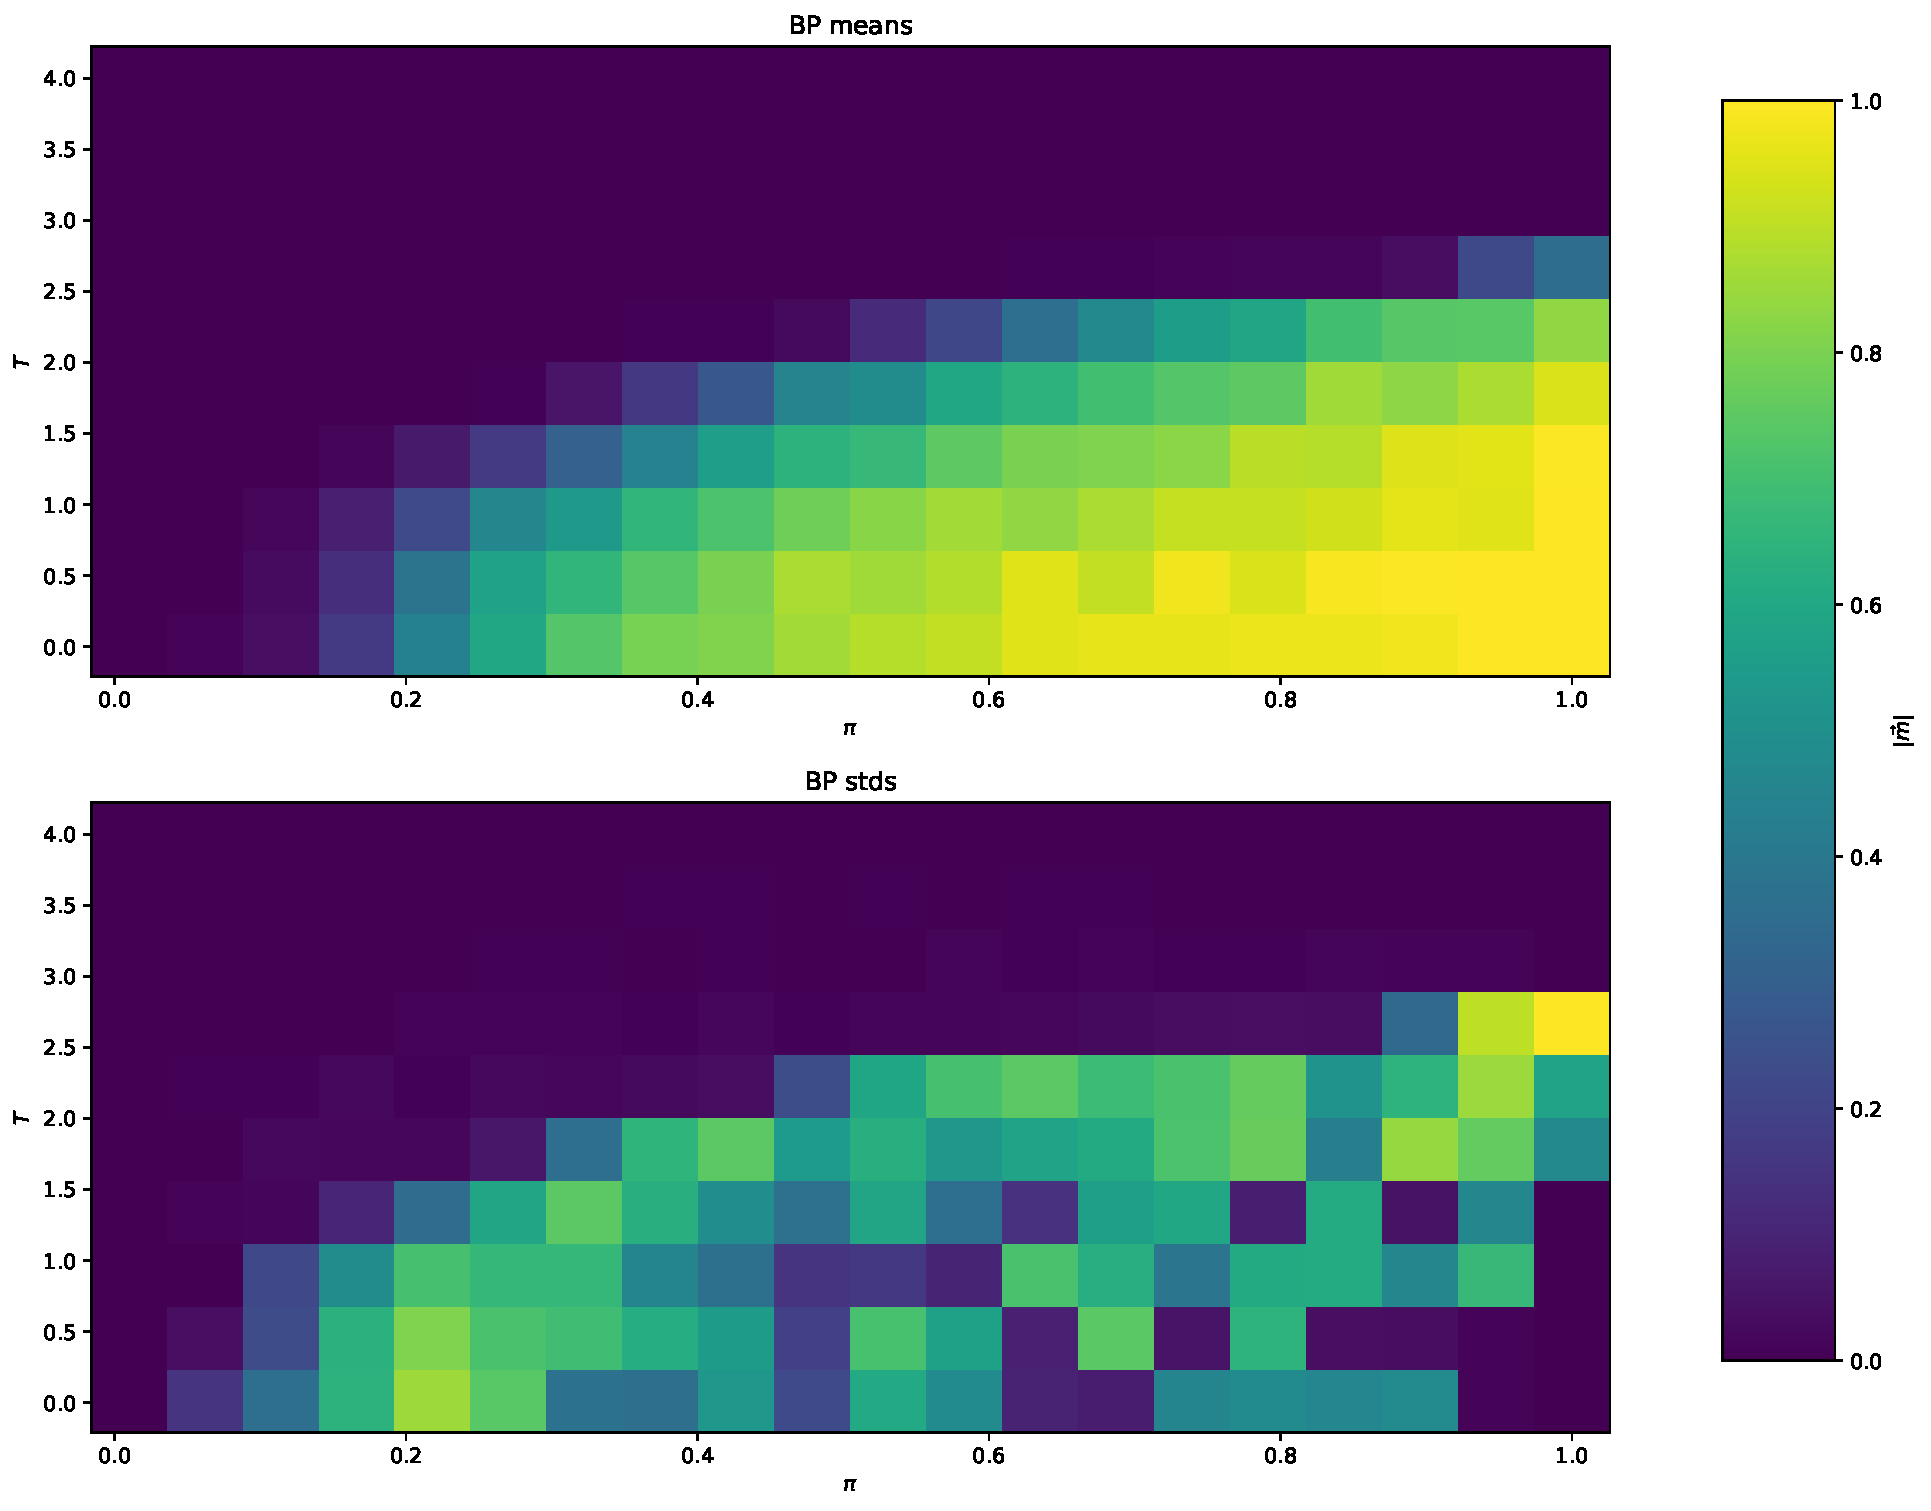
\includegraphics[width=.8\textwidth]{bp_heatmap}
        \caption{Heatmap for BP sampled magnetization means and stds}
        \label{fig:bp_heatmap}
    \end{figure}
\end{frame}

\begin{frame}{Population dynamics}
\end{frame}

\begin{frame}{Linear stability analysis and phase diagram}
    We know that the cavity fields have a distribution given by
    \begin{multline}
        \eta_{\text{cav}}(h) =
        \sum_{d=0}^{\infty} q_{d+1}
        \int \left( \prod_{k=1}^d \dd{h_k} \eta_{\text{cav}} (h_k) \right) \\
        \delta \left[ h - \frac{1}{2\beta} \sum_{k=1}^d
            \log\left( \frac{\cosh{\beta(h_k+1)}}{\cosh{\beta(h_k-1)}} \right)
        \right]
        \label{eq:cav_field_distrib}
    \end{multline}
    and also we know that the paramagnetic solution $\delta(h)$ is a
    \alert{fixed point} of the BP equations. We can perform a \alert{linear
    stability analysis} in order to understand how a small perturbation of the
    system affects its distribution.

    We shall be able to get also the phase diagram at the end of the analysis.
\end{frame}

\begin{frame}{Linear stability analysis}
    A small perturbation of the field is given by
    \begin{equation}
        \eta^{(0)} (h) = \delta(h-\epsilon_0)
    \end{equation}
    if we replace it in Eq.~\ref{eq:cav_field_distrib} we get that at the next
    iteration
    \begin{align}
        \epsilon_1 &= \int \dd{h} \eta^{(1)}(h) h\\
                   &= \sum_{d=0}^{\infty} q_{d+1} \frac{d}{2\beta} \log \left[
                       \frac{\cosh{\beta(\epsilon_0+1)}}{\cosh{\beta(\epsilon_0-1)}}
                   \right]\\
                   &\approx \sum_{d=0}^{\infty} q_{d+1} d \epsilon_0
                   \tanh{\beta}
    \end{align}
\end{frame}

\begin{frame}{Phase diagram}
    Recall that since the excess degree distributions are
    $$
    q_1 = \frac{1-\pi}{1+3\pi} \qquad q_4 = \frac{4\pi}{1+3\pi}
    $$
    then we can write
    \begin{align}
        \frac{\epsilon_1}{\epsilon_0} &= 3q_4 \tanh{\beta}\\
                                      &= \frac{12\pi}{1+3\pi} \tanh{\beta}
    \end{align}

    The system is \alert{stable} if the ratio is less than one, hence bringing
    us back to the \alert{paramagnetic} solution. Otherwise, the system will go
    in the ferromagnetic phase.

\end{frame}

\begin{frame}{Phase diagram}
    This means that we can draw the phase diagram, given that for $\epsilon_1 /
    \epsilon_0 = 1$ we get the critical line. It corresponds to the function
    $$
        T = \frac{1}{\arctanh \left( \frac{1+3\pi}{12\pi} \right)}
    $$
    that has an onset in
    $$
        \pi_0 = \lim_{T\to 0^+} \frac{1}{12\tanh{T^{-1}}-3} = \frac{1}{9}
    $$
    which is exactly the threshold for the onset of the giant component.
\end{frame}

\section{Inverse Ising model}

\begin{frame}{Inverse problem}
    Once we have a graph instance $G$ sampled from $\mathcal{G}$, and we have
    defined a spin model on the graph (e.g. a ferromagnetic Ising model), we
    might want to understand whether we are able to \alert{reconstruct} the
    topology of the graph (i.e. the edges) just by looking at the behaviour of
    the single components (i.e. the nodes).
    
    This task is hence that of estimating ``the rule'' once a set of data is
    given, and it is called an \alert{inverse problem}.
\end{frame}

\begin{frame}{Inverse problem}
    In particular we will construct the dataset as follows:
    \begin{itemize}
        \item Pick a random $G \in \mathcal{G}$
        \item Initialize spins over $G$ and perform an MCMC run in order to
            reach equilibrium at a temperature $T > T_c$ (\alert{paramgnetic}
            phase)
        \item Repeat this $M$ times in order to get $M$ samples of equilibrium
            spin configurations for $G$
    \end{itemize}

    Then we will attempt to perform inference over the dataset: in particular we
    will study its \alert{correlation matrix} and the \alert{naive mean field
    approximation inference}.
\end{frame}

\begin{frame}{Correlations}
    We can, first of all, look at correlations between components. Given the
    $\Sigma$ matrix of spin configurations (an $M \times N$ matrix), we can
    compute the \alert{correlation matrix}
    \begin{equation}
        C_{ij} = \expval{\sigma_i \sigma_j}_m - \expval{\sigma_i}_m
        \expval{\sigma_j}_m
    \end{equation}

    Then we can compute the \alert{positive predictive value} (PPV) by sorting
    the values of the correlation matrix in descending order, taking the
    greatest $n$ values and checking how many of the corresponding pairs of
    nodes are really connected by edges in the original graph.
    \begin{equation}
        \text{PPV}(n) = \frac{\#(i, j) \in E\text{ for }(i, j) \in n\text{-th
        ranking of highest correlations}}{n}
    \end{equation}
\end{frame}

\begin{frame}{Boltzmann machines}
    In order to perform network reconstruction on categorical variables (such
    our case, i.e. $\sigma_i=\pm 1$) we can use the \alert{Boltzmann machine}
    approach.

    By enforcing the maximisation of the log-likelihood over the \alert{fields}
    parameters $h_i$ and the {interactions} parameter $J_{ij}$ we get
    respectively the \alert{moment-matching} conditions between one- and
    two-points statistics of the data and the model. \cite[89]{spddm}

    \begin{align}
        \pdv{\mathcal{L}}{h_i} \reqeq 0 \quad &\Rightarrow \quad \mu_i =
        \expval{\sigma_i} \label{eq:mommatch1}\\
        \pdv{\mathcal{L}}{J_{ij}} \reqeq 0 \quad &\Rightarrow \quad \mu_{ij} =
        \expval{\sigma_i\sigma_j} \label{eq:mommatch2}
    \end{align}
\end{frame}

\begin{frame}{Boltzmann Machine Learning}
    Solving directly Equations~\ref{eq:mommatch1} and \ref{eq:mommatch2} is
    nontrivial, since finding the averages over the model distributions is hard.

    The problem can be recasted into an ML problem (\alert{Boltzmann machine
    learning}),
    where we would iteratively have $h_i$ and $J_{ij}$, and we would perform an
    MCMC run until equilibration, then we would update the parameters
    $$
    h_i^{t+1} = h_i^t + \eta_h (\mu_i - \expval{\sigma_i})
    $$
    $$
    J_{ij}^{t+1} = J_{ij}^t + \eta_J (\mu_{ij} - \expval{\sigma_i\sigma_j})
    $$
    and so on, for many epochs until we have learned the parameters.
    This amounts to a gradient descent process over the log-likelihood.

    This process still requires many MCMC runs and also explores a
    high-dimensional space, which makes the learning harder.
\end{frame}

\begin{frame}{Naive Mean Field Approximation}
    We might want to find an approximation in which we can express
    \alert{fields} and \alert{couplings} analytically.

    If we make a \alert{mean field} ansatz (i.e. the Boltzmann distribution
    factorizes in the sites) we can recast the problem of maximising a
    likelihood into that of inverting a matrix.

    In fact we can take the mean field free energy
    \begin{equation}
        G^{\text{mf}}(\vec m, J) = - \sum_{i<j} J_{ij} m_i m_j +
        \sum_i \left[ \frac{1+m_i}{2} \log \frac{1+m_i}{2} + \frac{1-m_i}{2}
        \log \frac{1-m_i}{2} \right]
        \label{eq:mf_free}
    \end{equation}
\end{frame}

\begin{frame}{Naive Mean Field Approximation}
    If we derive Eq.~\ref{eq:mf_free} twice wrt $m_i$ we get that the coupling
    matrix $J^{\text{mf}}_{ij}$ is equal to minus the inverse correlation matrix
    $[C]_{ij}^{-1}$, which is much easier to compute than the maximum
    log-likelihood.

    \begin{equation}
        J^{\text{mf}}_{ij} = - [C]_{ij}^{-1}
    \end{equation}

    Then we could compute the fields since $h_i^{\text{mf}}=\pdv{G}{m_i}$ hence
    \begin{equation}
    h_i^{\text{mf}} = -\sum_{j\neq i} J_{ij}^{\text{mf}} m_j + \arctanh{m_i}
    \end{equation}
    \cite[17]{inverse}
\end{frame}

\begin{frame}{Results for different dataset sizes}
    \begin{figure}
        \centering
        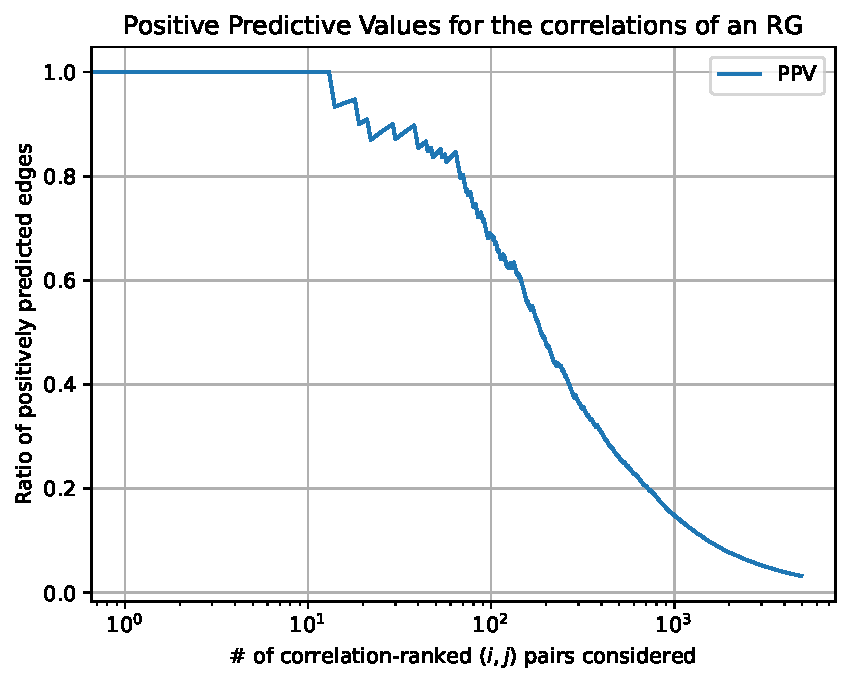
\includegraphics[width=.45\textwidth]{ppv_1h}
        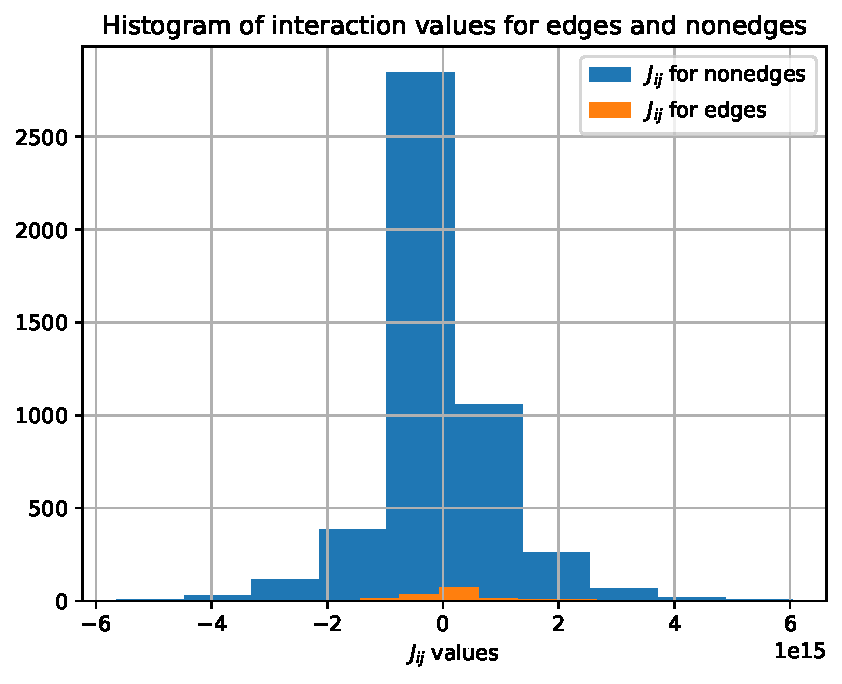
\includegraphics[width=.45\textwidth]{nmf_jhist_1h}
        \caption{PPV and distribution of $J$ values for $M=100$}
        \label{fig:nmf_1h}
    \end{figure}
\end{frame}

\begin{frame}{Results for different dataset sizes}
    \begin{figure}
        \centering
        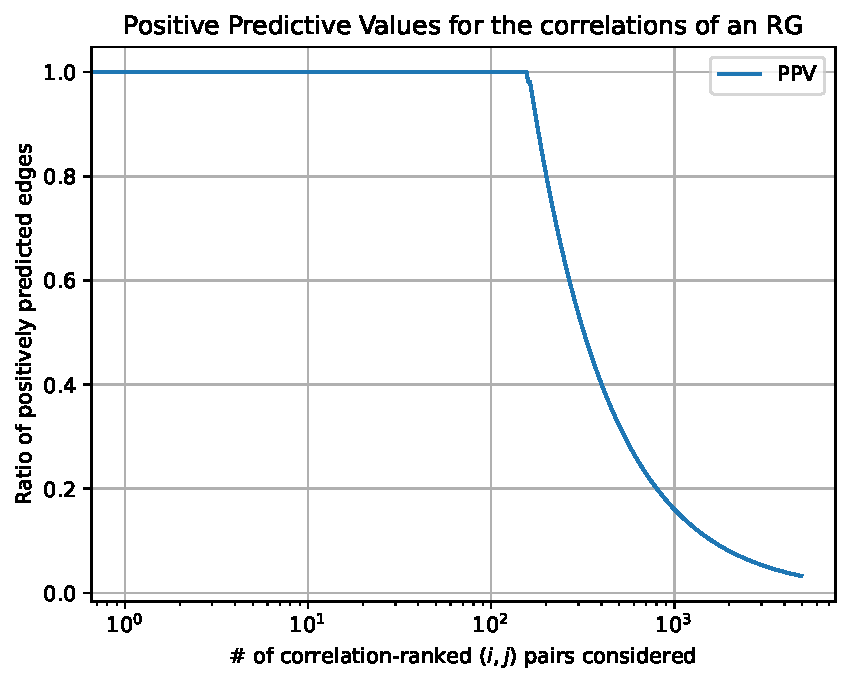
\includegraphics[width=.45\textwidth]{ppv_1k}
        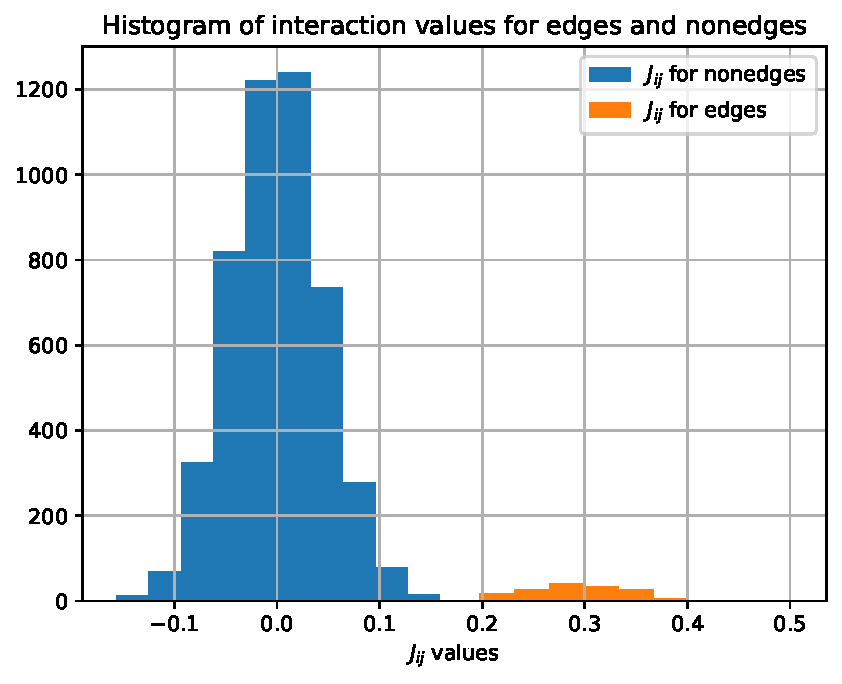
\includegraphics[width=.45\textwidth]{nmf_jhist_1k}
        \caption{PPV and distribution of $J$ values for $M=1000$}
        \label{fig:nmf_1k}
    \end{figure}
\end{frame}

\begin{frame}{Results for different dataset sizes}
    \begin{figure}
        \centering
        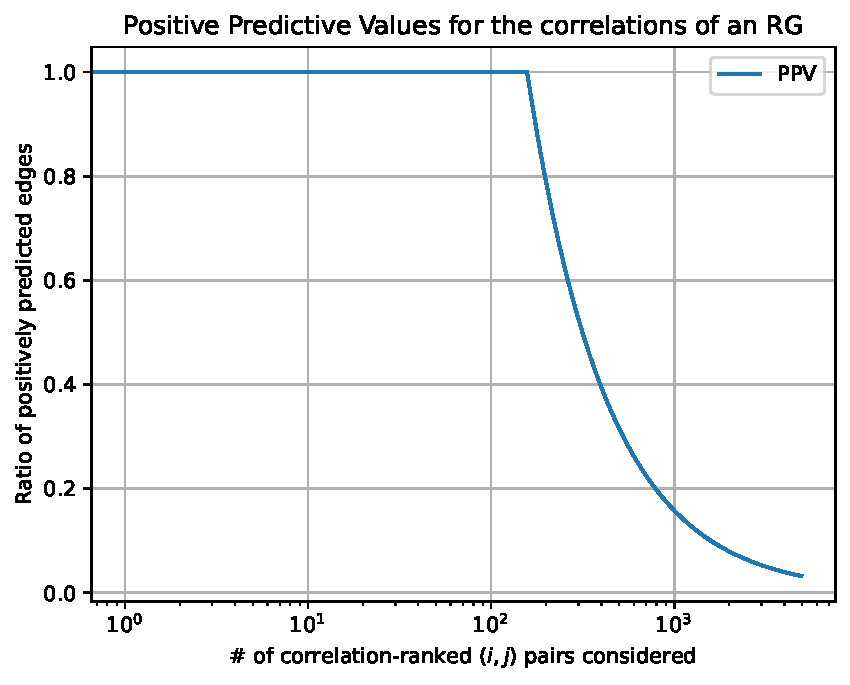
\includegraphics[width=.45\textwidth]{ppv_10k}
        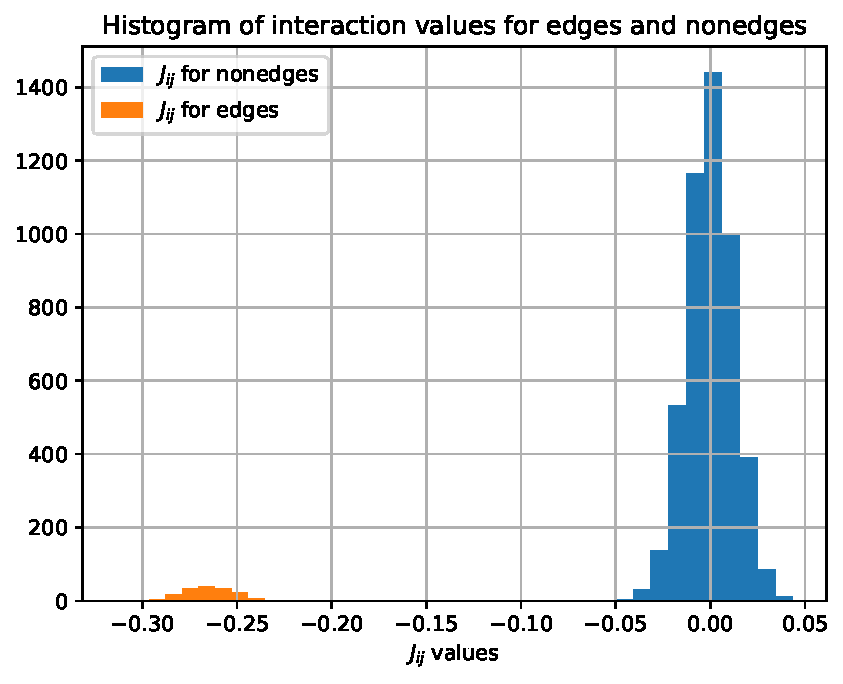
\includegraphics[width=.45\textwidth]{nmf_jhist_10k}
        \caption{PPV and distribution of $J$ values for $M=10000$}
        \label{fig:nmf_10k}
    \end{figure}
\end{frame}

\begin{frame}{Comments on inverse problem techniques}
\end{frame}

\section{Appendix}

\begin{frame}[allowframebreaks]{Bibliography}
    \printbibliography
\end{frame}

\end{document}
